\section{固体的燃烧}
\subsection{概述}
\subsection{燃煤锅炉}
\subsection{非均相反应}
\begin{enumerate}
    \item 反应物分子通过对流和(或)扩散作用到达固体表面;
    \item 反应物分子在固体表面被吸附;
    \item 包含被吸附分子、固体表面自身及气相分子的多种化合作用的基元反应;
    \item 产物分子在固体表面的解吸附;
    \item 产物分子通过对流和(或)扩散作用离开固体表面。
\end{enumerate}
三种反应模式:
\begin{enumerate}
    \item 如果反应物分子A的吸附能力较弱:\(\mathcal{R}=k(T)[\mathrm{A}]\);
    \item 如果A强吸附:\(\mathcal{R}=k(T)\);
    \item 如果A弱吸附、B强吸附:\(\mathcal{R}=k(T)\frac{[\mathrm{A}]}{[\mathrm{B}]}\)。
\end{enumerate}

\subsection{碳的燃烧}
\subsubsection{概述}
碳反应的总包反应,Power-law:
\begin{eqnarray}
    \mathrm{C + O_2} &\overset{k_1}{\rightarrow}& \mathrm{CO_2}\\
    \mathrm{2C + O_2} &\overset{k_1}{\rightarrow}& \mathrm{2CO}\\
    \mathrm{C+CO_2} &\overset{k_1}{\rightarrow}& \mathrm{2CO}\\
    \mathrm{C+H_2O} &\overset{k_1}{\rightarrow}& \mathrm{CO+H_2}
\end{eqnarray}

反应生成的主要产物CO扩散出去之后燃烧产生\(\mathrm{CO_2}\)。

在一定的条件下,颗粒内部扩散在碳的燃烧中发挥着重要的作用。但是在下面的分析中假定扩散无法通过固体表面。

\subsection{单模模型}
\textbf{假设}:
\begin{enumerate}
    \item 燃烧过程为准稳态;
    \item 球形碳颗粒在无限大的、静态的环境中燃烧;
    \item 在碳颗粒表面,碳与化学当量的氧气反应,产生二氧化碳;
    \item 气相仅由氧气、二氧化碳和惰性气体组成;
    \item \(k,c_p,\rho\mathcal{D}\)都为常数,路易斯数为1;
    \item 颗粒内部扩散可被忽略;
    \item 碳颗粒温度均匀,以灰体形式和外界环境辐射换热,而且没有中间介质的参与。
\end{enumerate}

\textbf{问题描述}:
求出碳的质量燃烧速率\(\dot{m}_C\)、表面温度\(T_s\)。这边只考虑组份及能量平衡方程。

\textbf{总的质量和组分守恒}:

流出去的质量流率恰好等于碳的燃烧速率。
\begin{eqnarray}
    \mathrm{1~kgC} + \nu_1 \mathrm{kg O_2}&\rightarrow& (\nu_1+1)\mathrm{kgCO_2}\\
    \nu_\mathrm{I} &=& \frac{21.999\mathrm{kgO_2}}{12.01\mathrm{kg}\mathrm{C}} = 2.664.
\end{eqnarray}
\begin{multicols}{2}
    \tiny
    \begin{figure}[H]
        \centering
        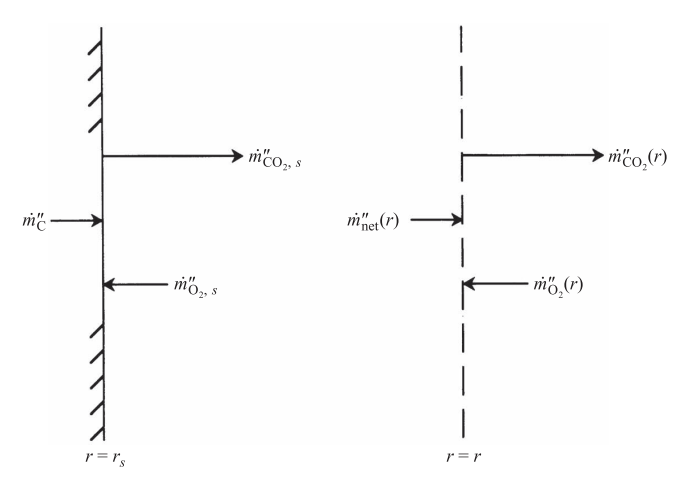
\includegraphics[width=.15\textwidth]{img/mass_flux_carbon.png}
    \end{figure}
    \begin{eqnarray}
        \dot{m}_\mathrm{O_2} &=& \nu_\mathrm{I} \dot{m}_\mathrm{C}\\
        \dot{m}_\mathrm{CO_2} &=& (\nu_\mathrm{I} + 1) \dot{m}_\mathrm{C}
    \end{eqnarray}
    然后在均匀相当中就可以运用菲克定律了。后面就是一通算。最后可以得到碳的通量:
\end{multicols}

\begin{equation}
    \dot{m}_\mathrm{C} = 4\pi r_s \rho \mathcal{D} \ln\left(\frac{1+Y_\mathrm{O_2,\infty}/\nu_\mathrm{I}}{1+Y_\mathrm{O_2,s}/\nu_\mathrm{I}}\right)
\end{equation}

\textbf{表面化学动力学}:认为碳和氧气的反应时一级的,可以进行一些计算,详见436
\textbf{电路比拟}
\begin{eqnarray}
    \dot{m}_\mathrm{C} &=& \frac{Y_\mathrm{O_2,\infty}-0.0}{R_\mathrm{kin}+R_\mathrm{diff}}\\
    R_\mathrm{kin} &\equiv& 1/K_\mathrm{kin} = \frac{\nu_\mathrm{I}R_u T_s}{4\pi r_s^2 MW_\mathrm{mix}k_c P}\\
    R_\mathrm{diff} &\equiv& \frac{\nu_\mathrm{I}+Y_\mathrm{O_2, s}}{\rho \mathcal{D}4\pi r_s}
\end{eqnarray}
\textbf{碳燃烧控制情况}

\begin{enumerate}
    \item \textbf{扩散控制}:\(R_\mathrm{kin}/R_\mathrm{diff}\ll1\):\(r_s\uparrow, T_s\uparrow, P\uparrow\);
    \begin{enumerate}
        \item 在\(k_c\)很大,快速的表面反应;
        \item 根据阿仑尼乌斯,这个时候温度很高;
        \item 也可能是碳表面上氧气浓度很小,接近于0.0,导致化学动力学参数中没有一个可以影响到燃烧速率。
    \end{enumerate}
    \item \textbf{化学动力学控制}:\(R_\mathrm{kin}/R_\mathrm{diff}\gg1\):\(r_s\downarrow, T_s\downarrow, P\downarrow\)。
    \begin{enumerate}
        \item \(R_\mathrm{diff}\)很小;
        \item \(Y_\mathrm{O_2,s}\)和\(Y_\mathrm{O_2,\infty}\)基本相等,表面氧气浓度比较大;
    \end{enumerate}
\end{enumerate}
\begin{equation}
    {\frac{R_{\mathrm{kin}}}{R_{\mathrm{diff}}}}\equiv\left({\frac{\nu_{1}}{\nu_{1}+Y_\mathrm{O_{2},s}}}\right)\left({\frac{R_{u}T_{s}}{M W_{\mathrm{mix}}P}}\right)\left({\frac{\rho \mathcal{D}}{k_{c}}}\right)\left({\frac{1}{r_{s}}}\right)
\end{equation}

\textbf{能量守恒}:一通算可以得到温度的分布,具体可以看440。

\begin{figure}[H]
    \centering
    \begin{subfigure}{.15\textwidth}
        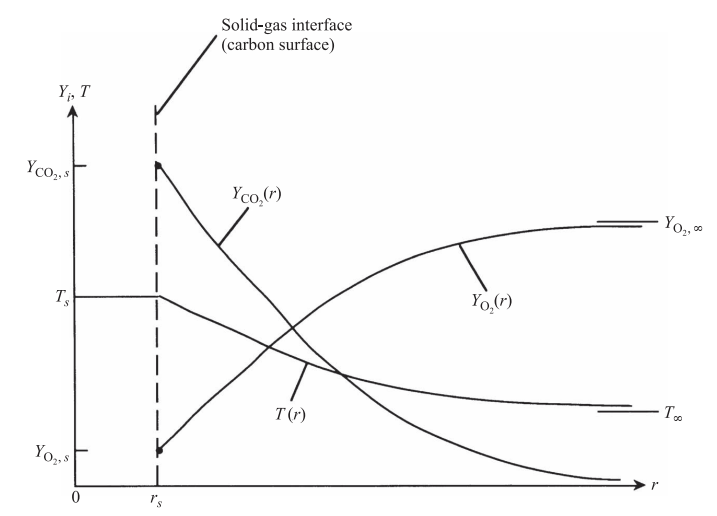
\includegraphics[width=.99\textwidth]{img/single_film.png}
        \caption{单模模型}
    \end{subfigure}
    \begin{subfigure}{.15\textwidth}
        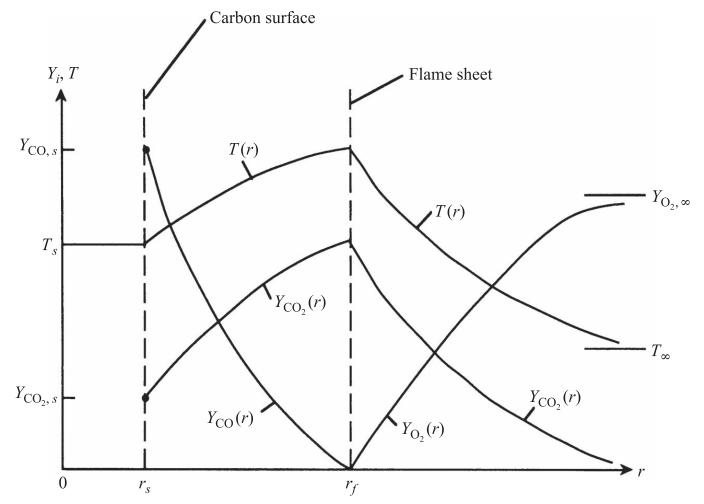
\includegraphics[width=.99\textwidth]{img/double_film.png}
        \caption{双膜模型}
    \end{subfigure}
\end{figure}

\subsubsection{双模模型}
\textbf{化学计量学}
\begin{eqnarray}
    \mathrm{1kgC}+\nu_s \mathrm{kgCO_2}&\rightarrow& (\nu_s+1)\mathrm{kgCO} \\
    \mathrm{1kgC}+\nu_f \mathrm{kg O_2} &\rightarrow& (\nu_f+1)\mathrm{kg CO_2}
\end{eqnarray}

其中
\begin{eqnarray}
    \nu_s &=& \frac{44.01}{12.01} = 3.664\\
    \nu_f &=& \nu_s - 1
\end{eqnarray}

然后我们就可以把各个组份的质量通量和碳的质量通量联系起来。

\textbf{组分守恒方程}:
应用菲克扩散定律可以获得分别描述内部区域和外部区域\(CO_\mathrm{2}\)分布的微分方程。单靠这个也不够,还需要利用化学动力学方程来对之进行封闭。

\textbf{表面化学动力学}:燃烧速率可以表达成与单膜反应中相同的形式,不过到他这儿是和二氧化碳反应生成一氧化碳。
\textbf{封闭性}

\subsubsection{碳颗粒燃烧时间}
依然是\(D^2\)定律,这里的燃烧速率:

\begin{equation}
    K_B = \frac{8\rho \mathcal{D}}{\rho_c}\ln(1+B)
\end{equation}

这里的传递数\(B\)对于单模选择\(B_\mathrm{O,m}\),对于双模选择\(B_\mathrm{CO_2, m}\)。
具体的计算可以看444页的例题。

忽略表面的化学动力学将会使燃烧速度有16.8 \%(=100\%(2.22-1.9)/1.9)的误差。表面温度(或压力)越低,动力学的影响就越大。 另外,随着燃烧的进行,\textit{颗粒直径也将不断减小,同样会使得动力学因素变得重要}。

\textbf{对流环境}:第十章的膜理论。

\subsection{煤的燃烧}
\subsubsection{煤的工业和元素分析}
\begin{figure}
    \centering
    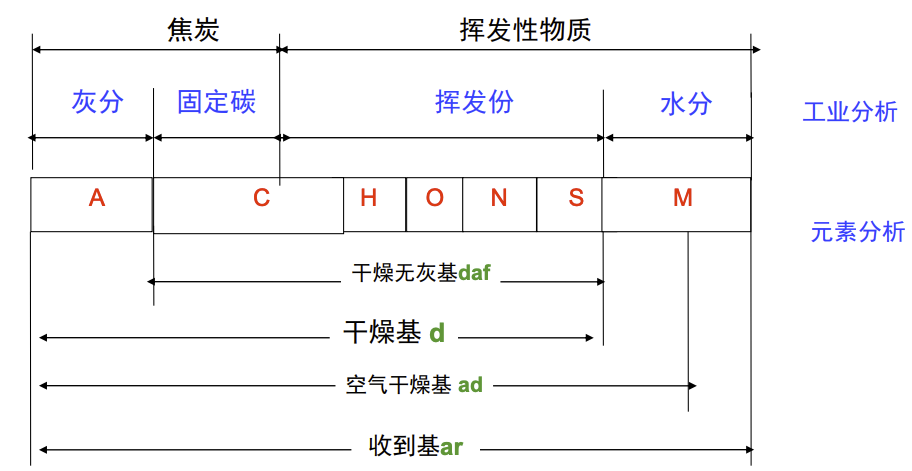
\includegraphics[width=.3\textwidth]{img/coal.png}
\end{figure}
\begin{enumerate}
    \item 收到基(应用基):以实际使用的煤为基准而测出的煤各元素的质量百分组成。
    \item 空气干燥基(分析基 ):以实验室使用的风干煤样(用温度为20\(^\circ\)C,相对湿度为70\%的空气)为基准而测出的煤各元素的质量百分组成。
    \item 干燥基:以无水的煤为基准而测出的煤各元素的质量百分组成。
    \item 干燥无灰基(可燃基 ):以无水、无灰的煤为基准而测出的煤各元素的质量百分组成。
\end{enumerate}

\subsubsection{煤的种类及特点}
\begin{enumerate}
    \item 褐煤:外观褐色,光泽黯淡。水分含量高,热值低,密度较小,含氧量高,化学反应强,极易氧化和自然。常作为加压气化燃料,锅炉燃料;
    \item 烟煤:挥发份含量高、灰分及水分较少,发热量高。可划分贫煤、焦煤、气煤。
    \item 无烟煤:挥发份含量低,燃点较高,燃烧时无粘结性。
\end{enumerate}